%%% Document class beamer, do not change
\documentclass[t]{beamer}
%% Optional packages
%\usepackage[utf8]{inputenc}
%% Required if you are writing in other language than English
\usepackage[finnish,swedish,english]{babel}
\usepackage{verbatim}
\usepackage{subfig}


%% Input the document information, note the use of short information in the footer
% The document title. Shows an example how linebreaks can be obtained.
\title[Lansing woods]{%
	Lansing woods
}

% The subtitle, e.g. the conference or course name.
% An abbreviation (or similar) in the short version is handy.
\subtitle[S-114.4202]{%
	S-114.4202 Special Course in Computational Engineering II
}
% The author names. Shows a second example of linebreaks.
% Note the use of \inst, see the \institute command!
\author[Väänänen]{%
	Ville Väänänen
}
% The authors' affiliations.
% Note the use of \inst, see the \author command!
\institute[Aalto University School of Science]{%
	Aalto University School of Science
}
% The date. Default date is \today.
%\date[Short Example Date]{%
%	Long Example Date, Default Date is \textbackslash today%
%}
% The subject. This is stored only in the PDF information.
\subject{Document Subject Example}

\usepackage{mylayout}

% Theme loading
\usetheme{Aalto}

%%% Begin the document
\begin{document}

%%% This file contains the code for the sample0x.tex files.

%% Create the title page
\maketitle

\begin{frame}
	\frametitle{Outline}
	\tableofcontents
	% You might wish to add the option [pausesections]
\end{frame}
\section{Data}

\begin{frame}
	\frametitle{Data}
	\vskip -30pt
	\begin{itemize}
  		\item Forest ecology data
  		\item Spatial locations $\in 282\times 282$m
  		\item Botanical classification
  		\item Lansing Woods, Clinton County, Michigan, USA, 1969 
	\end{itemize}
	\begin{centering}
		\includegraphics[width=0.7\textwidth]{lansing_map}
	\end{centering}
\end{frame}
	
	
	% You might wish to add the option [pausesections]
\frame[plain]{
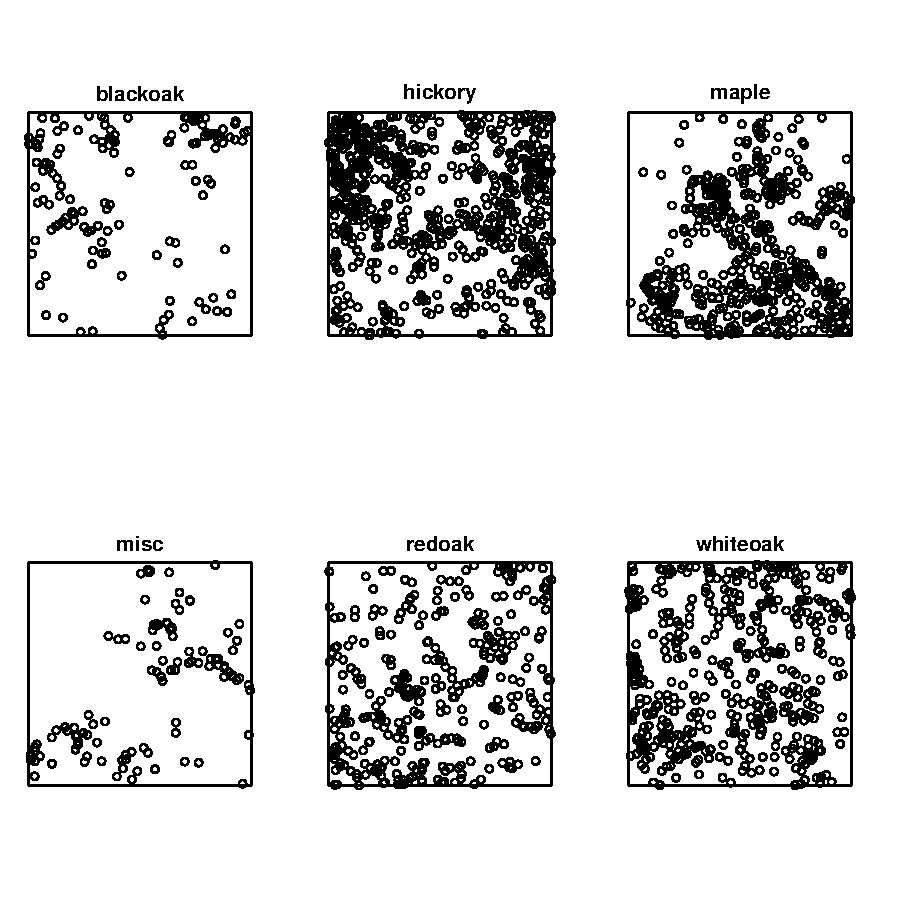
\includegraphics[width=0.9\textwidth]{lansing}
}

\begin{frame}
	\frametitle{Preprocessing}
	\begin{itemize}
  		\item Drop ``misc''
  		\item Combine oaks
  		\item Result:
  		\begin{itemize}
  			\item oak, $929$
  			\item hickory, $703$
  			\item maple, $514$
  		\end{itemize}
	\end{itemize}
\end{frame}


\frame[plain]{
	\begin{figure}[htb]
		  \centering
		  \subfloat[Maples]{\label{fig:maple}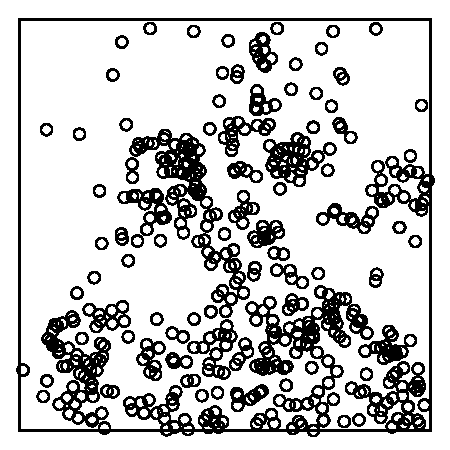
\includegraphics[width=0.3\textwidth]{lansing_maple}}
		  \subfloat[Hickories]{\label{fig:hickory}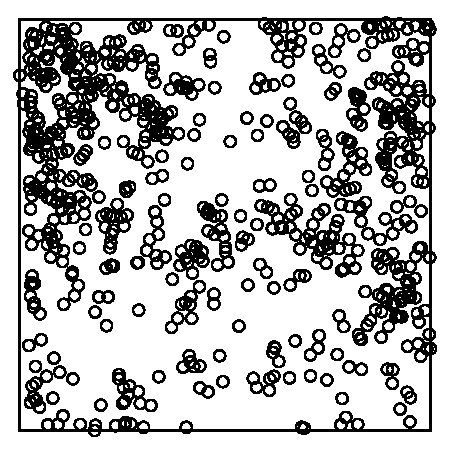
\includegraphics[width=0.3\textwidth]{lansing_hickory}}\\
		  \subfloat[Oaks]{\label{fig:oak}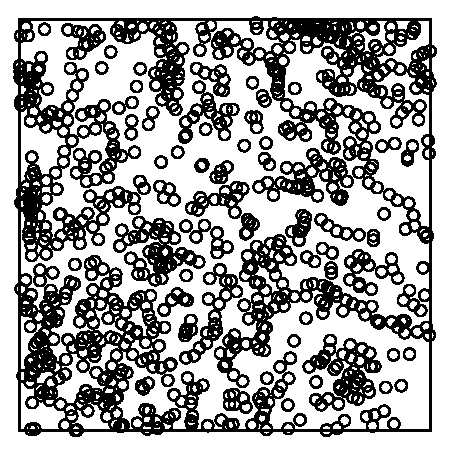
\includegraphics[width=0.3\textwidth]{lansing_oak}}
	  \label{fig:lansing_processed}
	\end{figure}
}

\section{Intensity}

\frame[plain]{
	\frametitle{Intensity}
	\vskip -40pt
	\begin{figure}[htb]
		  \centering
		  \subfloat[Maples]{\label{fig:int_maple}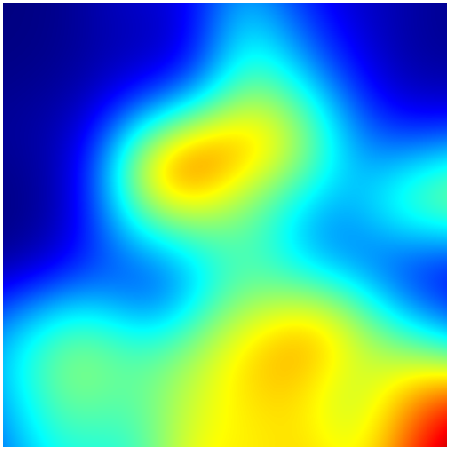
\includegraphics[width=0.27\textwidth]{intensity_relative_maple}}
		  \subfloat[Hickories]{\label{fig:int_hickory}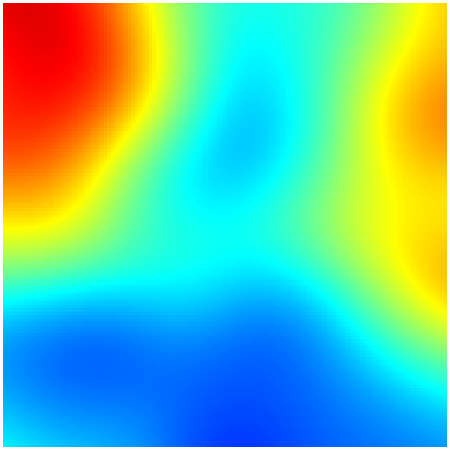
\includegraphics[width=0.27\textwidth]{intensity_relative_hickory}}\\
		  \subfloat[Oaks]{\label{fig:int_oak}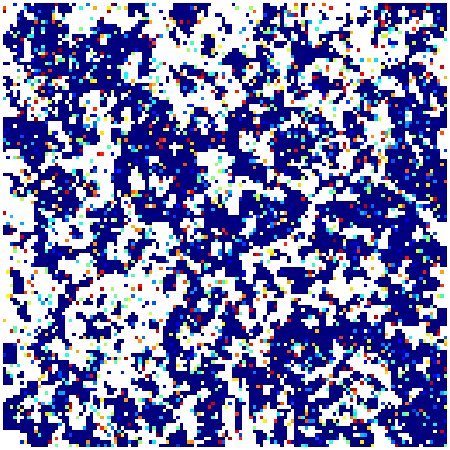
\includegraphics[width=0.27\textwidth]{intensity_relative_oak}}
	  \caption{Gaussian Kernel smoothed intensity estimates}
	  \label{fig:intensity_relative}
	\end{figure}
}
\frame[plain]{
	%\frametitle{Intensity}
\begin{figure}[htb]
	  \centering
	  \subfloat[All trees]{\label{fig:all_combined}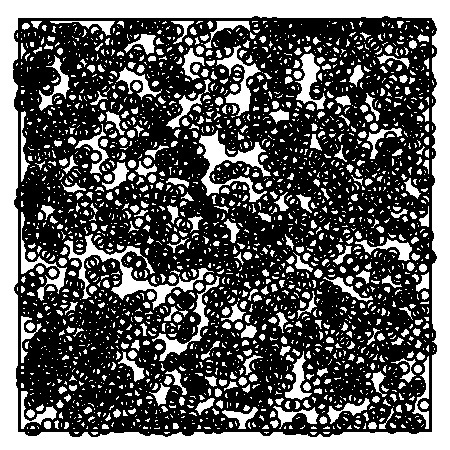
\includegraphics[width=0.27\textwidth]{lansing_combined}}
	  \subfloat[Oaks]{\label{fig:oaks_combined}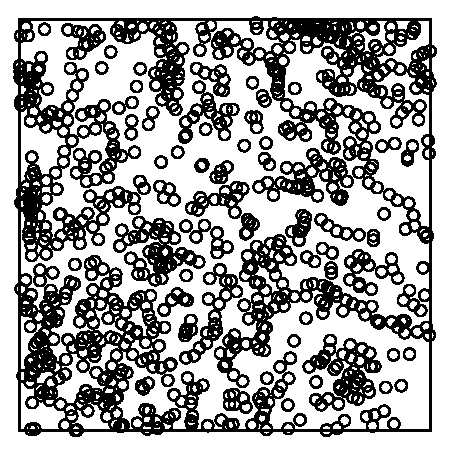
\includegraphics[width=0.27\textwidth]{lansing_oaks_combined}}\\
	  \subfloat[Hickories \& Maples]{\label{fig:hm_combined}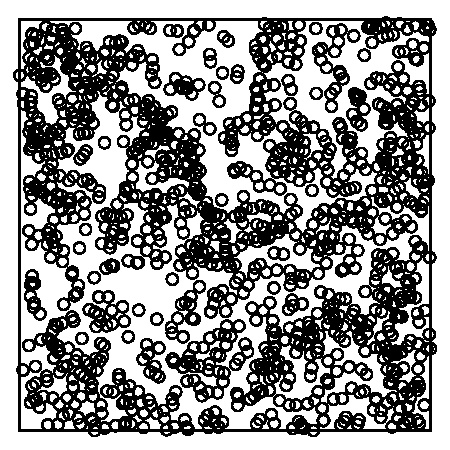
\includegraphics[width=0.27\textwidth]{lansing_hm_combined}}
  	\caption{Point patterns with different combinations of the marks in the dataset.}
	  \label{fig:combined_intensities}
\end{figure}
}

\section{Intra-species Interaction}

\begin{frame}
	\frametitle{Intra-species interaction}
	\vskip -55pt
\begin{figure}[htb]
	  \centering
	  \subfloat[Maples]{\label{fig:l_maple}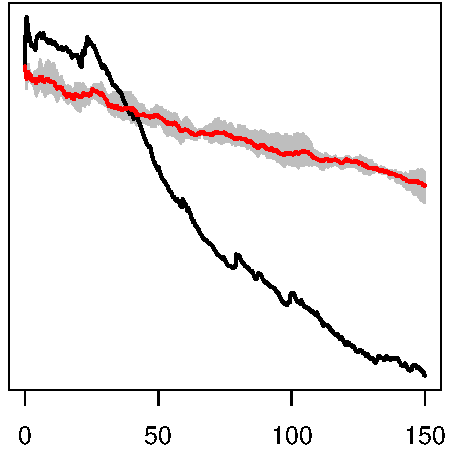
\includegraphics[width=0.35\textwidth]{l_maple}}
	  \subfloat[Hickories]{\label{fig:l_hickory}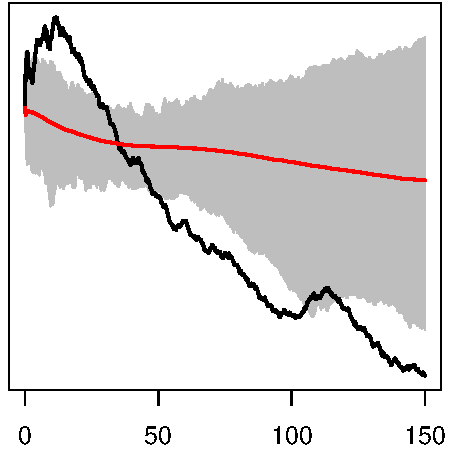
\includegraphics[width=0.35\textwidth]{l_hickory}}
	  \subfloat[Oaks]{\label{fig:l_oak}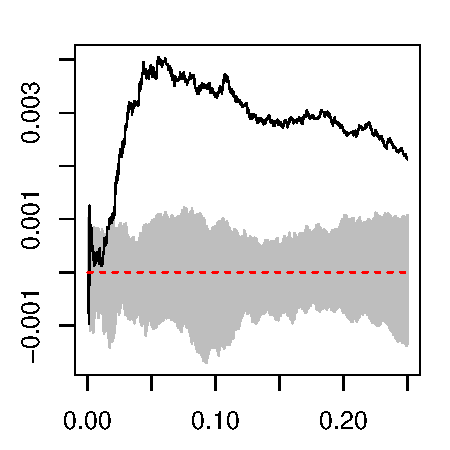
\includegraphics[width=0.35\textwidth]{l_oak}}
  \caption{Besag's L-function for the different species}
  \label{fig:intra_interactions}
\end{figure}
\end{frame}


\section{Inter-species Interaction}

\begin{frame}
	\frametitle{Inter-species interaction}
\vskip -55pt
\begin{figure}[htb]
	  \centering
	  \subfloat[Mark-connection function]{\label{fig:markc}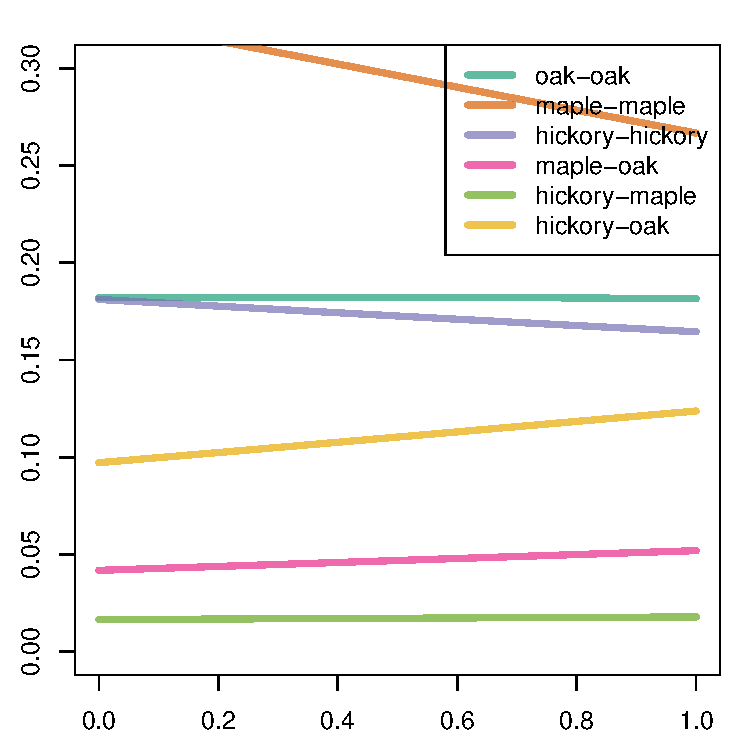
\includegraphics[width=0.52\textwidth]{markc}}
	  \subfloat[PPCF]{\label{fig:pcf}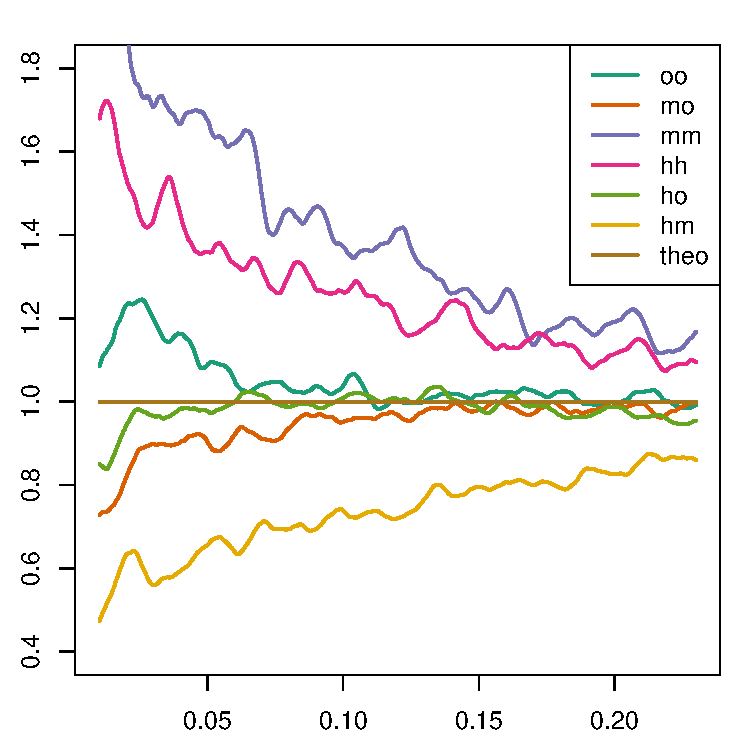
\includegraphics[width=0.52\textwidth]{pcf}}
  \label{fig:intra_interactions}
\end{figure}
\end{frame}

\section{Summary}

\begin{frame}
\frametitle{Summary}

\begin{itemize}
  \item Strong segregation between maples and hickories
  \item Some intra-species clustering
  \item Discarding the marks, homogenous intensity  
\end{itemize}

\end{frame}







\end{document}